\chapter{CLONAGEM DE CÓDIGO - ESTADO DA ARTE}

\section{Considerações iniciais}

Com a crescente demanda de softwares para suprir às necessidades geradas pelo avanço da tecnologia, a atenção ao modo como esses softwares são desenvolvidos é essencial. Clones de código-fonte são fragmentos de código replicados e a inserção clones em softwares ocorre por diversos motivos, entre eles estão novas funcionalidades, copiar e colar, e reutilização de código para uma determinada finalidade\cite{solanki2016comparative}.. Nesse sentido, diversas ferramentas e abordagens foram desenvolvidas para detectar clones de código-fonte em softwares visando, principalmente, impedir que mudanças inconsistentes possam  propagar erros e bugs, bem como auxiliar em manutenções necessárias. 

De modo a explorar tal contexto de detecção de clones, esse capítulo descreve um estudo empírico sobre clonagem de código em softwares. Assim sendo, a estrutura deste capítulo está da seguinte forma. A Seção 3.2 está a introdução do assunto acerca de ferramentas e abordagens existentes de detecção de clones. Na Seção 3.3 são abordados os tipos de clones bem como as técnicas comumente utilizadas para detectar clones em softwares. Seção 3.4 conta com a descrição de como foi feito o processo de mapeamento sistemático e o que ele objetiva responder. Na Seção 3.5 contém os resultados obtidos e a discussão acerca destes. Na Seção 3.6 está a discussão. Na Seção 3.7 consta os trabalhos relacionados. Na Seção 3.8 estão as ameaças a validade do trabalho. E, por último, na Seção 3.8 estão as considerações finais. 

\section{INTRODUÇÃO}
A clonagem de código é uma prática considerada comum e é introduzida por desenvolvedores principalmente na etapa de manutenção \cite{Fordos2016}\cite{Duala-Ekoko2007b}. Clones surgem por vários motivos, entre eles estão práticas de \textit{copy and paste}, inserção de funções semelhantes e reutilização de código \textit{ad-hoc} por programadores. A detecção de clones de código é essencial para prevenção da propagação de erros, correção de \textit{bugs}, manutenção e gerencia de sistemas de software \cite{petersen2008}\cite{solanki2016comparative}.

Clones podem ser idênticos ou possuir similaridades que também os classificam como tal. A similaridade pode ser classificada em dois grupos: i) sintática; e ii) semântica. Isso possibilitou a adoção da classificação de clones em quatro tipos, sendo os Tipos 1, 2 e 3 pertencentes ao primeiro grupo e o Tipo 4 pertencente ao segundo grupo \cite{Yuki2017}. Existem ferramentas desenvolvidas com o propósito de detectar clones em código. Essas ferramentas diferem principalmente em como fragmentos de código serão representados para serem comparados a outros fragmentos de código. Em geral, essa representação é por meio de \textit{String}, \textit{Token}, AST (\textit{Abstract Syntax Tree}), PDG (\textit{Program Dependence Graph}), Medidas e formas híbridas para chegar a uma abordagem final \cite{Schugerl2011}. Tal detecção pode ser feita analisando blocos de código, métodos, classes ou outra medida que determine, por exemplo, o tamanho do fragmento a ser analisado.

Diante da variedade de ferramentas, de técnicas, de métodos e de outras formas para detectar código clonado em sistemas de software, foi realizado um estudo exploratório, cujo resultado final obtido foi a identificação de 128 artigos que apresentam pesquisas sobre clonagem de código (ANEXO). Nesse estudo, foi utilizada a técnica Mapeamento Sistemático da Literatura (MSL), tendo em vista que os requisitos de pesquisa são menos rigorosos em relação à técnica Revisão Sistemática da Literatura (RSL), sendo o seu interesse em tendências de pesquisa \cite{kitchenham2010}. Em MSL, não precisa realizar avaliação de qualidade, pois o seu resultado é um inventário de artigos sobre a área temática, mapeados para uma classificação \cite{wieringa2006}, sendo uma visão geral do escopo da área que permite descobrir lacunas e tendências de pesquisa \cite{petersen2008}.

O restante desse trabalho está estruturado da seguinte maneira. Na Seção 2, o \textit{background} sobre clonagem de códigos, tipos de clonagem e técnicas de detecção de clones é apresentado. Na Seção 3, é detalhado o processo de planejamento do estudo exploratório que inclui questões e estratégias de pesquisa e critérios de inclusão e de exclusão. Na Seção 4, são apresentados os resultados obtidos no estudo exploratório. Na Seção 5, são discutidos esses resultados. Na Seção 6, estão resumidos alguns trabalhos relacionados. Na Seção 7, estão descritas ameaças a validade. Na Seção 8, são apresentadas conclusões e sugestões de trabalhos futuros.

\section{\textit{Background}}
A prática de ``copiar e colar'' trechos de código em outras partes do código é chamada de clonagem de código. Essa clonagem acontece em decorrência de vários fatores como reúso de código, necessidade de implementação de funções semelhantes, manutenção de sistemas legados ou acidentalmente por parte dos programadores \cite{solanki2016comparative}. À medida que o código aumenta de tamanho, a frequência com que a clonagem pode ocorrer tende a aumentar. Entretanto, estudos mostram que nem sempre o tamanho do código influencia na ocorrência de clones \cite{Torres2017}. Em sua maioria, tais ocorrências são relatadas em etapas de manutenção. Códigos clonados são classificados em quatro tipos acerca de sua similaridade sintática e semântica \cite{gautam2016various}\cite{solanki2016comparative}:

\begin{itemize}
	\item \textbf{Tipo 1 (\textit{exact clones})}. Fragmentos de código idênticos com variações de espaço, guias, \textit{layout} e comentários;
	
	\item \textbf{Tipo 2 (\textit{renamed/parameterized clones})}. Fragmentos de código com estrutura/sintaxe similar a outro(s) fragmento(s) de código, acrescidos de alterações em identificadores, literais, tipos, \textit{layout} e comentários;
	
	\item \textbf{Tipo 3 (\textit{near-miss clones})}. Fragmentos de código acrescidos de declarações, inserções/eliminações e alterações em identificadores, literais, tipos e \textit{layout};
	
	\item \textbf{Tipo 4 (\textit{semantic clones})}. Fragmentos de código funcionalmente semelhantes, mas não possuem semelhança textual. Ou seja, são funções do código original implementadas com sintaxe diferente.
\end{itemize}

Como exemplo desses tipos de clonagem, pode-se analisar um trecho de código hipotético (Código 1) e outros 4 trechos clonados dele, que apresentam modificações que caracterizam esses tipos. No trecho do Código 2, nas linhas 1 a 4, estão realçadas (cor de fundo diferente) informações que caracterizam o \textbf{Tipo 1} de clonagem, sendo espaçamento, adição de comentário, espaçamento e \textit{layout}, respectivamente.\\

\begin{scriptsize}
	\label{original}
	\estiloJava
	\begin{singlespace}
		\begin{lstlisting}[
		caption={Trecho original}, label=lst:javacode]
		ResultSet res = sist.executeQuery(query);
		boolean ok;
		for(ok = rs.first(); ok; ok = res.next()){
		results.add(new Project(res.getInt(2)));
		}
		return results;
		\end{lstlisting}
	\end{singlespace}
\end{scriptsize}

\begin{scriptsize}
	\label{tipo1}
	\estiloJava
	\begin{singlespace}
		\begin{lstlisting}[
		caption={Tipo 1 de Clonagem}, label=lst:javacode]
		ResultSet res(*@\hl{=}@*)sist.executeQuery(query);
		boolean ok; (*@\hl{//}@*)(*@\hl{Controlador}@*) 
		for(ok = rs.first(); ok; ok(*@\hl{=}@*)res.next())\{
		results.add(new Project(res.getInt(2))); (*@\hl{}@*) 
		return results;
		\end{lstlisting}
	\end{singlespace}
\end{scriptsize}

No Código 3, as linhas 1, 2, 3, 5 e 7 possuem alterações em identificadores de variáveis e, na linha 4, há alteração no \textit{layout}. Essas alterações caracterizam clonagem de código e classifica o Código 3 como \textbf{Tipo 2} de clonagem. No Código 4, o \textbf{Tipo 3} de clonagem pode ser identificado na linha 4, onde ocorre a eliminação da chamada do método \texttt{res.getInt(2)}. No Código 5, é possível verificar a mudança semântica no contexto de execução das instruções, onde o comando de repetição \texttt{for} foi subtituido pelo comando de repetição \texttt{do .. while}, sem alterações no resultado final.\\

\begin{scriptsize}
	\label{tipo2}
	\estiloJava
	\begin{singlespace}
		\begin{lstlisting}[
		caption={Tipo 2 de Clonagem}, label=lst:javacode]
		ResultSet (*@\hl{r}@*) = sist.executeQuery(query);
		boolean (*@\hl{ver}@*);
		for((*@\hl{ver}@*) = (*@\hl{r}@*).first(); (*@\hl{ver}@*); (*@\hl{ver}@*) = (*@\hl{r}@*).next())
		(*@\hl{\{}@*)
		(*@\hl{ok}@*).add(new Project(res.getInt(2)));
		}
		return ok;
		\end{lstlisting}
	\end{singlespace}
\end{scriptsize}

\begin{scriptsize}
	\label{tipo3}
	\estiloJava
	\begin{singlespace}
		\begin{lstlisting}[
		caption={Tipo 3 de Clonagem}, label=lst:javacode]
		ResultSet res = sist.executeQuery(query);
		boolean ok;
		for(ok = rs.first(); ok; ok = res.next()){
		results.add(new Project((*@\hl{ }@*));
		}
		return results;
		\end{lstlisting}
	\end{singlespace}
\end{scriptsize}

\begin{scriptsize}
	\label{tipo4}
	\estiloJava
	\begin{singlespace}
		\begin{lstlisting}[
		caption={Tipo 4 de Clonagem}, label=lst:javacode]
		ResultSet res = sist.executeQuery(query);
		boolean ok;
		(*@\hl{if(!res.first());}@*)
		(*@\hl{return results;}@*)
		(*@\hl{do\{ }@*)
		results.add(new Project(res.getInt(2)));
		(*@\hl{\} while(res.next()); }@*)    
		return results;
		\end{lstlisting}
	\end{singlespace}
\end{scriptsize}

Para a classificação dos tipos de clonagem ser feita de maneira adequada, técnicas de detecção foram elaboradas, nas quais a variação da representação do trecho de código a ser analisado é a principal diferença entre as técnicas mais comumente utilizadas \cite{Rattan2016}\cite{jang2009bitshred}:

\begin{itemize}
	\item \textbf{Baseada em texto (\textit{text-based})}. Técnica que consiste na combinação de textos e de \textit{strings} para encontrar candidatos a clones que diferem por meio de comentários e no \textit{layout} do(s) fragmento(s) de código a ser(em) analisado(s). Utilizando essa técnica, é possivel identificar clones do \textbf{Tipo 1}, cujos exemplos de abordagens de detecção são extração de texto e comparações mais distantes;
	
	\item \textbf{Baseada em símbolos (\textit{token-based})}. O processo de análise léxica tem como resultado a produção de uma sequência de \textit{tokens}. Esses \textit{tokens} são utilizados como parâmetros para métodos de busca para encontrar possíveis clones. Essa técnica pode ser utilizada para detectar clones do \textbf{Tipo 2};
	
	\item \textbf{Baseada em árvore (\textit{tree-based})}. \textit{Abstract Syntax Tree} (AST) fornece uma abstração da análise sintática em forma de árvore. A AST é percorrida por subárvores semelhantes até encontrar possíveis clones sintáticos contidos nessas subárvores, usando alguma técninca de correspondência de árvores. AST é utilizada na detecção, principalmente, de clones do \textbf{Tipo 3};
	
	\item \textbf{Baseada em grafo (\textit{graph-based})}. \textit{Graphy Dependence Program} (PDG) é um grafo direcionado e funciona como abstração semântica. Com a utilização do isomorfismo de um subgráfico obtido de um sistema de software, é possível encontrar subgráfos semelhantes, sendo classificados como clones. Também, é capaz de preservar a semântica original do código, sendo comumente utilizada para encontrar clones do \textbf{Tipo 4};
	
	\item \textbf{Baseada em híbrido (\textit{hybrid-based})}. Essa técnica consiste em combinar as técnicas anteriores, cujo objetivo é criar e/ou melhorar a detecção dos tipos de clone existentes.
\end{itemize}

Tais técnicas são implementadas de diversas formas. Para cada contexto de implementação, a(s) medida(s) a ser(em) utilizada(s) para comparação depende(m) da finalidade de utilização. Tamanho de fragmento, escopo de detecção, granularidade e escalabilidade são exemplos de medidas a serem utilizadas na implementação de ferramentas. Essas ferramentas detectam clones em várias linguagens e paradigmas, por exemplo, a ferramenta CCFinder \cite{Kamiya2002}. Em sua maioria, são implementadas para detecção em linguagens orientada a objetos (e.g., as linguagens de programação JAVA e C++) \cite{Kamiya2002}\cite{Lin2014}\cite{Yuan2011} ou para o paradigma procedural (e.g., a linguagem de programação C. Entretanto, a detecção de clones não se limita a tais paradigmas/linguagens.

\section{Planejamento do Estudo Exploratório}
Nesta seção, é descrito como o estudo exploratório, utilizando a técnica Mapeamento Sistemático da Literatura, foi planejado, incluindo a descrição das questões de pesquisa, escopo de pesquisa , estratégia de busca e critérios de classificação.

\subsection{Questões de pesquisa}
Nesse trabalho, o objetivo é realizar o estudo exploratório de pesquisas existentes, que abordam a detecção de códigos clonados em sistemas de software. É importante considerar a abrangência de informações que tal tema retorna e possibilitar que, com a definição e o estabelecimento do tipo de informações coletadas, forneçam às pesquisas futuras o estado da arte acerca da clonagem de código. Para tanto, foram coletadas informações sobre técnicas, processos, métodos, procedimentos, metodologias e ferramentas disponíveis na literatura que detectam código clonado em sistemas de software. Assim, foram elaboradas e respondidas as seguintes questões de pesquisa:
\newline

\begin{itemize}
	\item[\texttt{\textbf{Q1:}}] \texttt{Como é realizada a detecção de clones em código de sistemas de software?}
\end{itemize}
\noindent{\textbf{Justificativa}: Objetivo é mostrar o cenário de como são detectados clones em código. Assim sendo, identificar qual(is) ferramenta(s) é(são) utilizadas para identificar a existência de clones por parte dos programadores.}\\

\begin{itemize}
	\item[\texttt{\textbf{Q2:}}] \texttt{De que forma é realizada a detecção de clones nas abordagens que propõe técnicas, processos, métodos, procedimentos e metodologias para identificar clones?}
\end{itemize}
\noindent{\textbf{Justificativa}: O objetivo é coletar informações sobre o modo de abordar as formas de detecção de clones comuns às técnicas, processos, métodos, procedimentos e metodologias identificadas.}\\

\begin{itemize} \item[\texttt{\textbf{Q3:}}] \texttt{Quais tipos de clones são abordados nos artigos analisados?}
\end{itemize}
\noindent{\textbf{Justificativa}: O objetivo é identificar quais tipos de clonagem são identificados pelos autores e se existe realmente uma conveção da utilização desse termo, com base nos resultados obtidos.}\\

\begin{itemize}
	\item[\texttt{\textbf{Q4:}}] \texttt{Quais linguagens e paradigmas de programação são utilizados? }
\end{itemize}
\noindent{\textbf{Justificativa}: O objetivo é identificar as linguagens de programação comumente utilizadas para identificar clones e, com base nisso, quais paradigmas são predominantemente adotados pelos autores para realizar a detecção de clones em código.}\\

As respostas das questões de pesquisa Q3 e Q4 estão diretamente ligadas às respostas obtidas nas questões de pesquisa Q1 e Q2. 

\subsection{Estratégia de Pesquisa}
Após estabelecer as questões de pesquisa, foi possível definir palavras e/ou termos relevantes para obter resultados importantes e objetivos para o estudo exploratório. Como o foco está no contexto de clonagem de código, o termo ``Clone de Código'' é relevante. Para compor o contexto, foi necessário identificar os possíveis caminhos para chegar na resposta da questão de pesquisa Q1. Logo, ao decompor em termos tal questão, foram obtidas como resultado as variações das palavras-chave ``técnicas'', ``processos'', ``métodos'', ``procedimentos'', ``metodologias'' e ``ferramentas'' buscando abordar tal contexto. Além disso, ``software'' foi utilizada como a palavra-chave para a combinação final, pois representa o contexto de estudo. A combinação dessas palavras-chave com os conectores lógicos \texttt{AND} e \texttt{OR} forma a \textit{string} de busca utilizada:
\newline

\begin{center}
	\noindent\texttt{(``code clones'' OR ``cloned code'') AND (technique OR process OR method OR procedure OR methodology OR tool) AND (detect OR detection) AND software}
	\newline
\end{center}

Para responder às questões de pesquisa utilizando a \textit{string} de busca, foram selecionadas as bibliotecas digitais ACM \footnote{www.acm.org}, EI Compendex\footnote{www.engineeringvillage.com}, IEEE Xplorer\footnote{http://ieeexplore.ieee.org/}, Science Direct\footnote{www.sciencedirect.com}, Scopus\footnote{http://www.scopus.com} e Springer Link\footnote{www.link.springer.com}. Essas bibliotecas foram escolhidas por suportar (i) pesquisa avançada com utilização de palavras-chave, (ii) filtragem dos resultados por ano e área de publicação, (iii) filtragem por tipo de publicação e (iv) exportação do resultado da consulta em formato \texttt{BibTex} ou \texttt{Endnote}. O retorno inicial da pesquisa em cada biblioteca digital foi armazenado em bases de dados.

\subsection{Critério de Inclusão/Exclusão}
Na Tabela \ref{qntArtBase}, é apresentada a quantidade de trabalhos resultantes nas bibliotecas digitais. 

[CHEGAR NA UFLA E DESCREVER ISSO AQ]

Cada trabalho presente nas bases de dados passou por inspeções a fim de retirar os trabalhos caracterizados como não artigos (por exemplo, livros, normas e \textit{table of contents}) retornados na busca (Apenas Artigos), o que resultou em bases de dados com trabalhos considerados artigos, os quais foram reunidos em uma base de dados para serem removidos os artigos duplicados (Resultado Final). Nessa remoção, foi considerada a quantidade de palavras-chave, ou seja, o artigo duplicado e armazenado na biblioteca digital com menor quantidade de palavras-chave foi removido. Os artigos restantes foram lidos de modo que o foco da leitura se deu em identificar itens relacionados às questões de pesquisa.

\begin{table}[ht]
	\centering
	\caption{Quantidade de Artigos}
	\label{qntArtBase}
	\begin{tabular}{@{}lccc@{}}
		\toprule
		\multicolumn{1}{c}{Bibliotecas}    & Resultado        & Apenas      & Resultado     \\
		\multicolumn{1}{c}{Digitais}       & Inicial  & Artigos    &  Final \\
		\bottomrule
		ACM            & 119      & 82     & 27    \\
		EI COMPENDEX   & 196      & 61     & 19    \\
		IEEE           & 135      & 131    & 49    \\
		SCIENCE DIRECT & 35       & 34     & 2     \\ 
		SCOPUS         & 271      & 71     & 27    \\ 
		SPRINGER LINK  & 119      & 102    & 4     \\
		\bottomrule \toprule
		Total          & 875      & 481    & 128   \\ 
		\bottomrule
	\end{tabular}
\end{table}

Cabe ressaltar que três pesquisadores (Pesquisador A, Pesquisador B e Pesquisador C) foram envolvidos na obtenção dos artigos e foi realizado o seguinte procedimento:

\begin{enumerate}
	\item O Pesquisador A executou a \textit{string} de busca nas bibliotecas digitais selecionadas e documentou os resultados no sistema de software JabRef\footnote{http://www.jabref.org/};
	
	\item O Pesquisador A verificou e excluiu os trabalhos que não eram artigos e os artigos repetidos (com título, autores e resumo iguais). Na identificação de artigos repetidos, foram mantidos os artigos com palavras-chave que melhor descreviam o artigo;
	
	\item Os artigos encontrados foram avaliados pelo Pesquisador A e pelo Pesquisador B, de maneira individual e separada, quanto ao atendimento aos critérios de inclusão e de exclusão. Essa avaliação foi realizada por meio da leitura do título, do resumo e das palavras-chave. Os artigos, cujas avaliações causaram dúvidas quanto a sua inclusão/exclusão por parte dos pesquisadores, foram incluídos. Os artigos foram documentados em uma lista de artigos incluídos e excluídos com justificativa para sua inclusão ou exclusão;
	
	\item Realizou-se a interseção entre os artigos selecionados pelo Pesquisador A e pelo Pesquisador B, sendo esses artigos documentados (Interseção). Na ocorrência de algum desacordo sobre a inclusão ou a exclusão de artigos, os dois pesquisadores discutiram e resolveram. Em casos que não houve consenso, o artigo foi incluído. Os artigos excluídos foram documentados em uma lista de artigos excluídos com justificativa para sua exclusão;
	
	\item O Pesquisador C avaliou os artigos exluídos e as justificativas de exclisão e os artigos presentes na Interseção. O resultado foi o conjunto de artigos resultantes do estudo exploratório.
\end{enumerate}

\section{Resultados}
A finalização dos procedimentos e da seleção das informações necessárias, permite uma noção da diversidade de ferramentas e maneiras em comum de detecção de clones nas abordagens que propõe técnicas, processos, métodos , procedimentos e metodologias   acerca do estado da arte da detecção de clones em sistemas de software. A detecção de clones é abordada de diversas maneiras e por várias ferramentas que implementam essas abordagens, ambas identificadas nos 128 artigos obtidos após aplicar os critérios de inclusão/exclusão. Nesta seção, são apresentadas a análise das características gerais dos artigos resultantes do estudo exploratório, bem como respostas para as questões de pesquisa levantadas.

\subsection{Características Gerais dos Trabalhos Selecionados}
Como mencionado na seção 3, foram utilizadas 6 bibliotecas digitais de artigos científicos para a realização do estudo exploratório. Na Tabela \ref{qntArtBase}, é apresentada a quantidade final de 128 artigos como resultado para análise, sendo 27 artigos (21,09\%) na ACM, 19 artigos (14,84\%) na EI COMPENDEX, 49 artigos (38,28\%) na IEEE, 2 artigos (1,56\%) na SCIENCE DIRECT, 27 artigos (21,09\%) na SCOPUS e 4 artigos (3,12\%) na SPRINGER LINK. Foi considerado o período que engloba, aproximadamente, 18 anos de publicações (de 2001 a 2018) como mostra o gráfico da figura \ref{gAno}. A quantidade de artigos publicados acerca do tema ``Detecção de Código Clonado'', aparentemente, tende a crescer (gráfico da figura \ref{gAno}) com o decorrer dos anos. A maior concentração dessas publicações foram encontradas no ano de 2017, com o total de 17 artigos.

\begin{figure}[!htb]
	\centering
	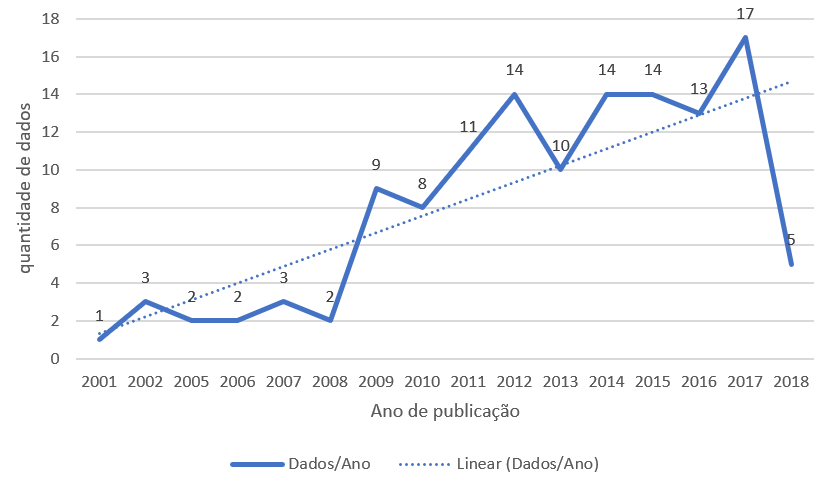
\includegraphics[height=2.2in, width=3in]{graficoAno.PNG}
	\caption{Quantidade ao longo dos Anos} 
	\label{gAno}
\end{figure}

Sobre a quantidade de pesquisadores, foram identificados 397 pesquisadores no tema ``Detecção de Clonagem de Código'', sendo os mais atuantes os pesquisadores \texttt{S. Kusumoto} com 7 artigos, \texttt{C. K. Roy} com 6 artigos, \texttt{Y. Higo} com 5 artigos e R. K. Tekchandani com 5 artigos. Cabe ressaltar a presença de dois grupos de pesquisadores que têm publicado juntos. Um desses grupos é composto por cinco pesquisadores \texttt{Nguyen, H. A.}, \texttt{Nguyen, T. N.}, \texttt{Nguyen, T. T.}, \texttt{Pham, N. H.} e \texttt{Al-Kofahi, J. M.} com 4 artigos (\texttt{ClemanX: Incremental clone detection tool for evolving software}, \texttt{Clone-Aware Configuratioan Management}, \texttt{Scalable and incremental clone detection for evolving software} e \texttt{Accurate and Efficient Structural Characteristic Feature Extraction for Clone Detection}. Outro grupo é composto por dois pesquisadores \texttt{Kanmani, S.} e \texttt{Kodhai, E.} com 4 artigos (\texttt{Detection of Type-1 and Type-2 Code Clones Using Textual Analysis and Metrics}, \texttt{Method-level code clone detection through LWH (Light Weight Hybrid) approach}, \texttt{Method-level incremental code clone detection using hybrid approach} e \texttt{Method-level code clone detection for Java through hybrid approach}).

Os 128 artigos selecionados no estudo exploratório foram publicados em 84 veículos distintos de divulgação científica, sejam \textit{journals}, \textit{workshops}, conferências e simpósios. Os quatro veículos com mais quantidade de artigos são \texttt{Symposium on Applied Computing (SP)} com 5 artigos publicados (5,85\%), \texttt{Asia-Pacific Software Engineering Conference (APSEC)} com 5 artigos publicados (5,85\%), \texttt{International Conference on Software Engineering (ICSE)} com 6 artigos publicados (7,14\%) e \texttt{International Workshop on Software Clones (IWSC)} com 8 artigos publicados (9,52\%) (Tabela \ref{journals}).

\begin{table}[ht]
	\centering
	%\scriptsize
	\caption{Principais Veículos de Publicação}
	\label{journals}
	\resizebox{\linewidth}{!}{
		\begin{tabular}{@{}ccc@{}}
			\toprule
			\textbf{Veículos de Divulgação Científica}              & \textbf{Qtde} & \textbf{Artigos}                                                               \\  \bottomrule \toprule
			Asia-Pacific Software Engineering Conference (APSEC)    & 5                   & A18, A07, A28, A97, A100
			\\\hline
			International Conference on Software Engineering (ICSE) & 6                   & A13, A33, A43, A65, A80, A11
			\\\hline
			International Workshop on Software Clones (IWSC)        & 8                   & \begin{tabular}[c]{@{}l@{}}A20, A27, A44, A73, A82, A87,\\   A96, A98\end{tabular}
			\\\hline
			Symposium on Applied Computing (SP)                     & 5                   & A19, A26, A45, A78, A49
			\\\bottomrule                                                       
		\end{tabular}
	}
\end{table}

\subsection{Resposta às Questões de Pesquisa}
Em resposta a questão de pesquisa Q1
\newline

\begin{center}
	\fbox{
		\parbox{7cm}{
			\centering \texttt{Como é realizada a detecção de clones em código de sistemas de software?} } }
	\newline
\end{center}

\noindent{a detecção de clones é feita por meio de abordagens e feramentas que implementam essas abordagens. Foram identificadas 52 ferramentas (Tabela \ref{ferramentas}). Cada ferramenta utiliza uma representação de fragmentos a serem analisados/considerados clone (Tabela \ref{ferramentas}), sendo \textit{Token}, Árvore (ou AsT) e Grafo as representações que possuem mais quantidade de ferramentas.}

\begin{table}[ht]
	\scriptsize
	\caption{Ferramentas Identificadas}
	\label{ferramentas}
	\begin{tabular}{@{}ccc@{}}
		\toprule
		\textbf{Ferramenta }   & \textbf{Baseada em }                     & \textbf{Referência }  \\ \bottomrule \toprule
		CCCD          & Análise Concólica               & A72
		\\ \hline
		CLORIFI       & Análise Concólica               & A57
		\\\hline
		Asta          & Árvore                          & A23
		\\\hline
		CCLearner     & Árvore                          & A79
		\\\hline
		CCR           & Árvore                          & A99
		\\\hline
		ClemanX       & Árvore                          & A17
		\\\hline
		Clever        & Árvore                          & A35
		\\\hline
		CReN          & Árvore                          & A42
		\\\hline 
		Deckard       & Árvore                          & A11
		\\\hline 
		KLON          & Árvore                          & A121
		\\\hline 
		LICCA         & Árvore                          & A4
		\\\hline 
		RefactoreRL   & Árvore                          & A58
		\\\hline
		MultiDup      & Árvore e Medidas                & A1
		\\\hline
		CloneDR       & AST                             & A75
		\\\hline
		SHAPE         & Extração de Procedimento Amorfo & A22
		\\\hline
		CCSharp       & Grafo                           & A38
		\\\hline
		ClemanX       & Grafo                           & A33, A125
		\\\hline
		CloneWorks    & Grafo                           & A25
		\\\hline
		CMCD          & Grafo                           & A18
		\\\hline
		DyCLINK       & Grafo                           & A36
		\\\hline
		GemScan       & Grafo                           & A125
		\\\hline
		SCVD          & Grafo                           & A50
		\\\hline
		Scopio        & Grafo e Híbrida                 & A81
		\\\hline
		DebCheck      & Híbrida                         & A21
		\\\hline
		PC Detector   & Híbrida                         & A95
		\\\hline
		SynTex        & Híbrida                         & A44
		\\\hline
		Hanni         & Macros                          & A30
		\\\hline
		HeapAbsCC     & Manipulação de \textit{Heap}    & A60
		\\\hline
		gCad          & Mapeamento de Função            & A103
		\\\hline
		Clone Miner   & Medidas                         & A94
		\\\hline
		SDD           & Medidas                         & A6
		\\\hline
		XIAO          & Medidas                         & A9, A27
		\\\hline
		JCC           & \textit{Pipeline}               & A111
		\\\hline
		CCDemon       & Recomendação Interativa         & A55
		\\\hline 
		BinClone      & \textit{Token}                  & A89
		\\\hline 
		BOREAS        & \textit{Token}                  & A70
		\\\hline 
		CCFinder      & \textit{Token}                  & A7, A13, A14
		\\\hline 
		CCFinderSW    & \textit{Token}                  & A97
		\\\hline
		Ctcompare     & \textit{Token}                  & A24
		\\\hline
		FRISC         & \textit{Token}                  & A63
		\\\hline
		IDCCD         & \textit{Token}                  & A100
		\\\hline
		LSC Miner     & \textit{Token}                  & A124
		\\\hline
		ReDeBug       & \textit{Token}                  & A78
		\\\hline 
		RTF           & \textit{Token}                  & A41
		\\\hline
		SaCD          & \textit{Token}                  & A62
		\\\hline
		ScalClone     & \textit{Token}                  & A53
		\\\hline
		SHINOBI       & \textit{Token}                  & A66
		\\\hline
		SourcererCC   & \textit{Token}                  & A90
		\\\hline
		SourcererCC-1 & \textit{Token}                  & A90
		\\\hline
		VUDDY         & \textit{Token}                  & A49
		\\\hline 
		Simone        & Não Informado                   & A123
		\\\hline
		VFDTECT       & Não Informado                   & A88
		\\\hline
		\toprule
		\textbf{Total de Ferramentas }& &52 \\
		\bottomrule
	\end{tabular}
\end{table}

Em resposta a questão de pesquisa Q2
\newline

\begin{center}
	\fbox{
		\parbox{7cm}{
			\centering \texttt{De que forma é realizada a detecção de clone nas abordagens que propõe técnicas, processos, métodos, procedimentos e metodologias para identificar clones?} } }
	\newline
\end{center}

\noindent{foram identificadas várias formas de detectar clones. Tais formas foram agrupadas em 26 técnicas (Tabela \ref{tecnicas}) que se baseiam na representação do código para detectar clones, sendo a técnica baseada em Árvore (AST e Distância) a que possui mais quantidade de artigos que a utiliza. Ao todo, 124 artigos apresentaram a detecção de clones baseadas nos tipos listados na tabela \ref{tecnicas} (os artigos A91, A116, A119 e A123 não apresentaram). Mesmo que possuam algum tipo de interface implementada, algoritmos e outros, 71 trabalhos (55,42\%) não possuem nome para as abordagens descritas pelo próprios autores para referenciá-las. Por esse motivo, os resultados são em relação ao tipo de representação (baseada em) utilizada para detecção de clones. Não foi identificada a técnica abordada em três artigos (A12, A88, A123).}

\begin{table*}[h]
	\centering
	\scriptsize
	\caption{Técnincas Detecção de Código Clonado}
	\label{tecnicas}
	\resizebox{\linewidth}{!}{
		\begin{tabular}{@{}lccc@{}}
			\toprule
			\textbf{Técnica Baseada em }            & \textbf{Métodos mais Utilizados}                                     & \textbf{Quantidade} & \textbf{Referência}                                                                                            \\ \bottomrule \toprule
			Texto                          & Verificação de \textit{string}                                       & 1          & A92                                                                                                   \\\midrule
			Token                          & Comparação de \textit{tokens} e distância                            & 19         &  \begin{tabular}[c]{@{}l@{}}A7, A13, A14, A24, A32, A41, A49, A53, A62, A63, A66, A70, A78, A88, A89, A90, A97, A100, A124                  \end{tabular}  \\\hline
			Árvore                         & AST e Distância                                             & 27         & \begin{tabular}[c]{@{}l@{}}A1, A4, A11, A17, A23, A28, A31, A34, A35, A37, A39, A42, A45, A47, A48, A58, A61, A67, A73, A75, A79, A83,\\ A93, A99, A112, A121, A125, A126 \end{tabular}\\\hline
			Grafo                          & PDG, Vetores e Distância                                    & 14         &  \begin{tabular}[c]{@{}l@{}}A18, A25, A33, A36, A38, A43, A50, A54, A64, A76, A80, A81, A102, A125 \end{tabular}                                      \\\hline
			Híbrida                       &AST, PDG e Medidas   & 19        & \begin{tabular}[c]{@{}l@{}}A2, A8, A9, A10, A16, A19, A21, A44, A46, A74, A95, A98, A101, A106, A107, A108, A110, A115, A127 \end{tabular}                                                  \\\hline
			Métrica                        &   Tamanho, Complexidade, Escalabilidade, etc                                       & 19         & \begin{tabular}[c]{@{}l@{}} A1, A3, A6, A15, A27, A29, A40, A56, A77, A82, A87, A92, A94, A105, A109, A114, A115, A122, A128          \end{tabular}                               \\\hline
			Macro                          & Macros                                                      & 1          & A30                                                                                                   \\\hline
			Procedimento Amorfo            & Procedimentos Amorfos                                       & 1          & A22                                                                                                   \\\hline
			Análise Concólica              & Teste Simbólico                                          & 3          & A26, A57, A72                                                                                         \\\hline
			Recomendação Interativa        & Recomendação Interativa                                     & 1          & A55                                                                                                   \\\hline
			Semântica Baseada na Web       &   Web Semântica                                                          & 5          & A5, A20, A84, A85, A86                                                                                \\\hline
			Processo Hierárquico Analítico &   Tomada de Decisões Complexas                                                          & 1          & A51                                                                                                   \\\hline
			Fechamento Transitivo          &   Fecho Transitivo                                                          & 1          & A52                                                                                                   \\\hline
			Análise de Crescimento         &   Análise de Crescimento                                                          & 1          & A59                                                                                                   \\\hline
			Manipulação de \textit{Heap}            &    \textit{Heap}                                                         & 1          & A60                                                                                                   \\\hline
			Métodos Formais                &   Formalismo Matemático                                                          & 2          & A65, A96                                                                                              \\\hline
			Limiar                         &   Limite                                                          & 1          & A68                                                                                                   \\\hline
			PALEX                          &  PALEX                                                           & 1          & A69                                                                                                   \\\hline
			\textit{Wavelets}                       &  Decompor e Descrever ou Representar 
			outra Função/Dados                                                         & 1          & A71                                                                                                   \\\hline
			Mapeamento de Função
			
			&  Mapear Funções em Estruturas de Dados                                                         & 1          & A103                                                                                                  \\\hline
			Aprendizado de Máquina
			
			&   Aprendizado de Máquina                                                        & 1          & A104                                                                                                  \\\hline
			\textit{Pipeline}
			&   Ações Paralelas                                                         & 1          & A111                                                                                                   \\\hline
			Controle de \textit{Statements} & Controle de Fluxo de \textit{Statements} & 1   & A113      \\\hline
			Chave de Redução & Elemento Principal de Redução & 1   & A117      \\\hline
			Índice  & Índice de Referência & 1   & A118      \\\hline
			Mineração de Conjunto 
			& Itens Frequentemente Ponderados & 1   & A120      \\
			\bottomrule \toprule
			\textbf{Total de Técnicas }&& &26 \\
			\bottomrule
		\end{tabular}
	}
\end{table*}

Em resposta a questão de pesquisa Q3,
\newline

\begin{center}
	\fbox{
		\parbox{7cm}{
			\centering \texttt{Quais tipos de clones são abordados nos artigos analisados?} } }
	\newline
\end{center}

\noindent{quanto aos tipos de clones, todos foram listados e relacionados na Tabela \ref{tp} e, quando o tipo não estava explicitamente identificado, havia referência somente à detecção de clones semânticos ou sintáticos. Foram identificadas 155 ocorrências de abordagens de detecção de clones, sendo 37 artigos detectam clones do Tipo 1, 37 artigos detectam clones do Tipo 2, 44 artigos detectam clones do Tipo 3, 11 artigos detectam clones do Tipo 4, 14 artigos detectam clones semânticos e 12 artigos detectam clones sintáticos.}

\begin{table}[ht]
	\scriptsize
	\caption{Tipos de Clones Identificados}
	\label{tp}
	\begin{tabular}{@{}ccc@{}}
		\toprule
		\textbf{Tipo}      & \textbf{Quantidade} & \textbf{Referência}                                                                                                                                                                                                                       \\\bottomrule \toprule
		1         & 37         & \begin{tabular}[c]{@{}l@{}}A6, A8, A14, A16, A18, A24, A26, A30, A32, A34, A38,  A39, A45,\\ A46, 
			A49, A59, A62, A71, A77, A79, A81, A82, A92, A96, A97, A98,\\ A99, A103, A105, A106, A107, A108, A109, A113, A118, A120.\end{tabular}
		\\\hline
		2         & 37         & \begin{tabular}[c]{@{}l@{}}A6, A8, A14, A18, A24, A26, A31, A34, A38, A39, A43, A45, A46,\\ A49, A53, A59, A62, A71, A77, A79, A81, A82, A83, A91, A92, A96,\\ A97, A98, A99, A103, A105, A106, A107, A108, A113, A118, A120\end{tabular}
		\\\hline
		3         & 44         & \begin{tabular}[c]{@{}l@{}}A1, A6, A8, A2, A8, A14, A16, A18, A19, A22, A25, A26, A29, A34,\\ A37, A38, A39, A41, A42, A43, A45, A46, A47, A63, A68, A70, A71,\\ A73, A74, A75, A79, A81, A82, A85, A90, A94, A97, A99, A03, A105,\\ A106, A107, A113, A117, A120 \end{tabular}
		\\\hline
		
		4         & 11         & \begin{tabular}[c]{@{}l@{}}A2, A14, A20, A26, A38, A39, A46, A72, A74, A79, A97, A113 \end{tabular}
		\\\hline
		
		Semântico & 14          & \begin{tabular}[c]{@{}l@{}}A4, A11, A28, A80, A84, A86, A87, A93, A95, A102, A112, A119, A124,\\ A126 \end{tabular}
		\\\hline
		Sintático & 12          & A10, A60, A69, A78, A83, A100, A101, A110, A115, A116, A21, A127
		\\\toprule
		\textbf{Total  } &155 & \\
		\bottomrule
	\end{tabular}
\end{table}

Em resposta a pergunta Q4,
\newline

\begin{center}
	\fbox{
		\parbox{7cm}{
			\centering \texttt{Quais linguagens e paradigmas de programação são utilizados?} } }
	\newline
\end{center}

\noindent{foram identificadas 13 linguagens de programação (Tabela \ref{ling}). A quantidade de vezes em que elas apareceram nos artigos está distribuidas em Python (1), JavaScript (1), C\# (12), Java (62), C++ (21), C (43), Modula 2 (1), Scheme (1) , Cobol (3), Erlang (3), Haskell (1), Ruby (2) e Fortran (1). Essas linguagens pertencem a 6 paradigmas de programação (Figura \ref{paradigmas}): i) estrutural; ii) imperativo; iii) funcional; iv) orientado a objetos; v) procedural; e vi) concorrente.}

\begin{table}[ht]
	\centering
	\scriptsize
	\caption{Linguagens de Programação Identificadas}
	\label{ling}
	\resizebox{\linewidth}{!}{
		\begin{tabular}{@{}ccc@{}}
			\toprule
			\textbf{Linguagens de Programação} & \textbf{Qtde} &\textbf{ Artigos}                                                                                                                                                                                                                                                                             \\ \bottomrule \toprule
			Python                    & 1          & A73
			\\\hline
			JavaScript               & 1          & A4
			\\\hline
			C\#                      & 12         &\begin{tabular}[c]{@{}l@{}} A1, A9, A19, A23, A24, A27, A29, A31, 45, A59, A91,\\ A105     \end{tabular}                                           
			\\\hline
			Java                     & 62         & \begin{tabular}[c]{@{}l@{}}A2, A4, A7, A8, A10, A11, A15, A18, A19, A23, A25, \\ A26, A28, A29, A32, A33, A35, A36, A37, A39, A42,\\ A43, A44, A45, A47, A52, A55, A57, A62, A64, A65,\\ A68, A69, A70, A71, A74, A75, A79, A82, A84, A85,\\ A91, A92, A94, A96, A98, A99, A100, A101, A106,\\ A107, A108, A109, A110, A111, A112, A113, A117,\\ A118, A119, A120, A126    \end{tabular}
			\\\hline
			C++                      & 21         & \begin{tabular}[c]{@{}l@{}}A3, A7, A8, A9, A15, A16, A27, A31, A40, A49, A50, \\ A52, A62, A66, A57, A78, A80, A81, A94, A110, A113 \end{tabular}
			\\\hline
			C                        & 43         & \begin{tabular}[c]{@{}l@{}}A3, A4, A7, A9, A11, A15, A19, A21, A22, A25, A26,\\ A27, A29, A31, A34, A37, A38, A40, A45, A49, A50,\\ A52, A60, A62, A63, A66, A69, A75, A76, A77, A78,\\ A80, A81, A83, A85, A92, A104, A106, A108, A113,\\ A116, A118, A121\end{tabular}
			\\\hline
			Modula 2                 & 1          & A4
			\\\hline
			Scheme                   & 1          & A4
			\\\hline
			Cobol                    & 3          & A7, A15, A30
			\\\hline
			Erlang                   & 3          & A46, A58, A61
			\\\hline
			Haskell                  & 1          & A48
			\\\hline
			Ruby                     & 2          & A69, A91
			\\ \hline
			
			
			Fortran  &1  &A121  \\ \bottomrule \toprule
			
			\textbf{Número total de linguagens}  &  & 13
			\\\bottomrule
		\end{tabular}
	}
\end{table}

\begin{figure}
	\centering
	\scriptsize
	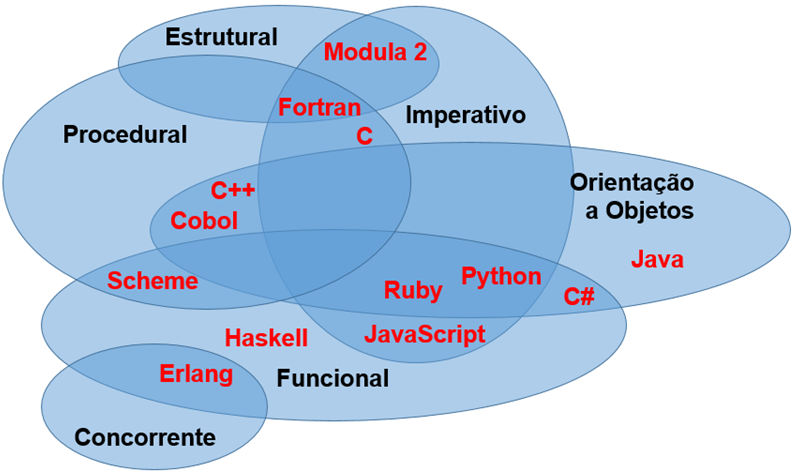
\includegraphics[height=2.2in, width=3in]{Linguagens.png}
	\caption{Paradigmas de Programação Identificados} 
	\label{paradigmas}
\end{figure}

\section{Discussão}
Clones de código são detectados por abordagens e ferramentas, sendo implementadas de maneiras diferentes. Porém, é possível identificar algumas maneiras de compará-los, por exemplo, o modo em que o código a ser dito ``clone'' é representado para identificação e os tipos de clones identificados. Os trabalhos selecionados no estudo exploratório possuem intervalo de publicação de 18 anos (de 2001 a 2018), inclusive.

Quanto à quantidade de veículos de divulgação científica identificados (84 \textit{journals}, \textit{workshops}, conferências e simpósios), pode ser considerada alta e mostra a diversidade de contextos/áreas da Engenharia de Software, onde são abordadas a detecção de clones, por exemplo, segurança, inteligência artificial, engenharia reversa, \textit{data mining} e computação aplicada. É observável que a maior concentração de artigos foram apresentados no \texttt{International Workshop on Software Clones (IWSC)}, cujo objetivo é ``reunir pesquisadores e profissionais para avaliar o estado atual da pesquisa, discutir problemas comuns e direções emergentes (como a detecção de clones em modelos de software, análise de clones em reengenharia para reutilização, análise de clones em evolução de software e detecção de clones em direitos autorais e plágio)''\footnote{https://iwsc2018.github.io/}.

Foram reunidas abordagens e suas bases de representação similar em tipos diferentes. Alguns desses tipos são comumente encontrados na literatura como árvores e grafos, cujos resultados foram obtidos em maior quantidade, e outras são representações relativamente novas, pois apresentam uma abordagem com uma base de identificação completamente diferente das usuais, por exemplo, \textit{wavelets}, métodos formais e análise concólica, as quais apresentam bom desempenho e escalabilidade na detecção de clones complexos comparados a outras abordagens. Entretanto, algumas dessas técnincas não são explicadas adequadamente pelos autores e/ou passaram por poucas avaliações.

As ferramentas facilitam a identificação de clones para os programadores. Elas comumente oferecem interfaces para visualização dos clones identificados, sejam elas gráficas ou não. Além disso, conseguem identificar clones de vários tipos e isso os beneficia, pois identificá-los manualmente é cansativo, dispendioso e propenso a falhas. Nem todas essas ferramentas de detecção são explícitas quanto a isso ou garantem encontrar um tipo de clone específico, o que acaba por generalizar termos como clones semânticos e sintáticos. Tal convenção pode gerar confusão quanto aos tipos identificados, pois não existe uma exatidão dos tipos que abrange cada termo.

Quanto aos tipos identificados nota-se divergência entre os autores quanto à utilização ou não da classificação usual que ditam 4 tipos de clones relacionados às similaridades semântica e sintática. Com isso, alguns autores preferem utilizar a nomenclatura convencional de separação, sendo os tipos de clones diferidos por similaridades sintáticas e semânticas.

Mesmo com a variedade de linguagens de programação existentes, é perceptível que, em clonagem de código, destaca-se a utilização de programas desenvolvidos em JAVA (40\%), C (27,92\%) e C++ (13,63\%). Tais valores podem estar relacionados à popularidade de utilização da linguagem em diversas outras áreas de pesquisa. Isso também revela o porquê da maioria das abordagens existentes empregarem suas técnicas em ambientes voltados ao desenvolvimento utilizando o paradigma orientado a objetos e procedural. 

Também, pode-se perceber, no decorrer da leitura, que os artigos são comumente aplicados em contextos industriais e acadêmicos. No contexto industrial, a detecção de clones em sistemas de software trata principalmente da realização de testes nesses sistemas, visando às melhorias de manutenção. No contexto acadêmico, relativamente maior que o industrial, são destacadas pesquisas buscando o desenvolvimento de ferramentas que proporcionam mais escalabilidade e desempenho. Outros aspectos comumente abordados juntamente com a detecção de clones são (i) refatoração de códigos clonados (com o objetivo de manutenção) e (ii) necessidade/propensão a gerência de clones.

Relatados, em sua maioria, no conteúdo dos artigos analisados, clones de código têm impacto direto na manutenção de sistemas de software. A detecção por meio de ferramentas e abordagens busca facilitar a sua identificação pelos programadores, a fim de reduzir propagações de erros disseminados por clones não identificados, bem como facilitar inserções/alterações/remoções de funções em sistemas de software.

\section{Trabalhos Relacionados}
Em um trabalho \citeauthor{roy2007survey}, realizam um estudo do estado da arte, criando um \textit{survey} sobre detecção de clones. Assim sendo, em parte desse trabalho, a literatura sobre clones de código é abordada, bem como a identificação de ferramentas e de técnicas de detecção de clones, descrevendo o processo. Neste trabalho, foi relatado quais ferramentas e abordagens existem, utilizando investigação da literatura bem como características relacionadas à linguagem e ao paradigma de programação.

Em outro trabalho \citeauthor{gautam2016various}, são classificados técnicas de detecção de clones e tipos de clones com pesquisas que abrangem, por típo de técnincas, períodos diferentes de publicação, em até, no máximo, o ano de 2012. Neste trabalho, são identificadas essas abordagens no período de 2001 a 2018.

Em outro trabalho \citeauthor{kapdan2014structural}, é tratado o problema de identificação de clones estruturais, considerando abordagens de detecção de clones baseadas em medidas, utilizando pesquisa sobre o estado da arte. Neste trabalho, são identificadas ferramentas/abordagens que utilizam medidas, mas não especificá-las.

\section{Ameaças a validade}
As ameaças a validade deste estudo exploratório são importantes para determinar o nível de confiança dos dados obtidos.

\textbf{\textit{String} de busca}. A \textit{string} de busca pode conter falhas ou estar incompleta para o contexto, o que pode gerar alteração no resultado obtido nas buscas nas bibliotecas digitais utilizadas.

\textbf{Obtenção de material}. A \textit{string} de busca pode conter falhas, a falta de termos ou excesso deles pode comprometer a qualidade dos dados. 

\textbf{Conteúdo analisado}. Vários trabalhos analisados não fundamentam completamente (ou nenhuma vez) como/com base em que são as técnicas de detecção utilizadas bem como os Tipos de clones identificados pela ferramenta/abordagem criada. Dados acerca da linguagem e paradigma de programação utilizada também é uma lacuna a ser preenchida com informações não contidas nos trabalhos selecionados.

\section{Considerações Finais}

Clones de código são trechos de código idênticos ou similares que têm alta propensão à propagação de erros, \textit{bugs} e a geração de inconsistências em sistemas de software. Se um trecho é modificado por algum motivo e seu clone não, o processo de manutenção tende a tornar-se mais trabalhoso e massante, principalmente, tratando-se de sistemas de software mais complexos. Logo, ferramentas e abordagens relacionadas à detecção de clones são construídas visando minimizar esses problemas e auxiliar os programadores.

Esse capítulo do trabalho apresentou um estudo exploratório utilizando a técnica Mapeamento Sistemático de Literatura sobre a detecção de códigos clonados, no nível de código, em sistemas de software. Foram analisados e coletados dados de 128 artigos relacionados ao tema para responder as questões de pesquisa. Esse resultado foi obtido por um processo detalhado de investigação/exploratório descrito na Seção 3.

Algumas informações foram identificadas a respeito das características gerais identificadas nos artigos selecionados. Em relação às bibliotecas digitais, em ordem descrescente, a quantidade de artigos analisados estão concentradas na IEEE (38,28\%), ACM (21,09\%), SCOPUS (21,09\%), EI COMPENDEX (14,84\%), SPRINGER LINK(3,12\%) e SCIENCE DIRECT (1,56\%). Com relação ao ano de publicação, foi abrangido o período de 2001 a 2018, onde a maior concentração de publicações foi no ano de 2017. Quanto aos autores, quatro autores principais destacaram-se com publicações superiores/iguais a cinco artigos. Além disso, foram identificados dois grupos de pesquisadores que têm publicado em conjunto; um grupo com cinco pesquisadores que publicaram quatro artigos juntos e outro grupo com dois pesquisadores que publicaram quatro artigos juntos. Também, foi contabilizado ao todo 84 veículos de divulgação de trabalhos científicos diferentes, categorizando a diversificação de aplicação da detecção de clones.

Como resposta à questão de pesquisa Q1, como resultado foram encontradas 52 ferramentas implementadas baseadas em 12 tipos diferentes. Para a questão de pesquisa Q2, o total de técnicas utilizadas para encontrar cada tipo de clone quantificam 26 modos diferentes. Foram encontrados os quatro tipos de clone ao final do estudo das ferramentas e das abordagens analisadas, respondendo a questão de pesquisa Q3. Para a questão de pesquisa Q4, foram identificadas 13 linguagens de programação diferentes e 6 paradigmas.

Como trabalhos futuros, é sugerida a pesquisa sobre as ferramentas desenvolvidas para gerenciar a detecção de clones, visto que pode facilitar a utilização pelos programadores. Além disso, pesquisar as medidas utilizadas em cada abordagem para melhor compreendê-las. 


\begin{table*}[b]
	\begin{flushleft}
		\begin{tabular}{l}
			\textbf{\fontsize{11}{1.5}\selectfont{ANEXO - ARTIGOS IDENTIFICADOS NO ESTUDO EXPLORATÓRIO}}
		\end{tabular}
	\end{flushleft}
\end{table*}

\begin{table*}[ht]
	\scriptsize
	\centering
	\caption{Artigos Selecionados}
	\label{artigosselecionados}
	\resizebox{\linewidth}{!}{
		\begin{tabular}{cllc}
			\toprule
			\textbf{ID}   & \textbf{Título}                                                                                                                                         &\textbf{ Autores(as)}                                                                                                                & Fonte                                                     \\ \bottomrule \toprule
			A1  & Detection of near-miss clones using metrics and abstract syntax trees                                                                & Vishwachi; Gupta, Sonam                                                                                               & EI COMPEDEX                                               \\\hline 
			A2  & Semantic Clone Detection Using Machine Learning                                                                                      & Sheneamer, A.; Kalita, J.                                                                                             & IEEE                                                      \\\hline 
			A3  & Identifying clones in the Linux kernel                                                                                               & Casazza, G.; Antoniol, G.; Villano, U.; Merlo, E.; Penta, M. Di                                                       & IEEE                                                      \\\hline 
			A4  & LICCA: A tool for cross-language clone detection                                                                                     & Vislavski, T.; Rakić, G.; Cardozo, N.; Budimac, Z.                                                                   & IEEE                                                      \\\hline 
			A5  & An approach to identify duplicated web pages                                                                                         & Lucca, G. A. Di; Penta, M. Di; Fasolino, A. R.                                                                        & IEEE                                                      \\\midrule
			A6  & SDD:   High Performance Code Clone Detection System for Large Scale Source Code                                                      & Lee, Seunghak; Jeong, Iryoung                                                                                         & ACM                                                       \\\hline 
			A7  & On detection of gapped code clones using gap locations                                                                               & Ueda, Y.; Kamiya, T.; Kusumoto, S.; Inoue, K.                                                                         & EI COMPEDEX                                               \\\midrule
			A8  & Clone detection using time series and dynamic time warping techniques                                                                & Abdelkader, M.; Mimoun, M.                                                                                            & IEEE                                                      \\\hline 
			
			A9  & XIAO: Tuning Code Clones at Hands of Engineers in Practice                                                                           & Dang, Yingnong; Zhang, Dongmei; Ge, Song; Chu, Chengyun; Qiu, Yingjun; Xie, Tao                                       & ACM                                                       \\\hline 
			A10  &\begin{tabular}[c]{@{}l@{}} To enhance the code clone detection algorithm by using hybrid approach for detection\\ of code clones\end{tabular}                                & Roopam; Singh, G.                                                                                                     & IEEE                                                      \\\hline 
			A11  & DECKARD: Scalable and Accurate Tree-Based Detection  of Code Clones                                                                  & Jiang, L.; Misherghi, G.; Su, Z.; Glondu, S.                                                                          & IEEE                                                      \\\hline 
			A12  & A Code clone oracle                                                                                                                  & Krutz, Daniel E.; Le, Wei                                                                                             & EI COMPEDEX                                               \\\hline 
			A13  & Detecting Differences Across Multiple Instances of Code Clones                                                                       & Lin, Yun; Xing, Zhenchang; Xue, Yinxing; Liu, Yang; Peng, Xin; Sun, Jun; Zhao, Wenyun                                 & ACM                                                       \\\hline 
			A14  & \begin{tabular}[c]{@{}l@{}}CCFinder:  a multilinguistic token-based code clone detection system for large scale\\ source code  \end{tabular}                                   & Kamiya, T.; Kusumoto, S.; Inoue, K.                                                                                   & IEEE                                                      \\\hline 
			A15  & Software clone detection using clustering approach                                                                                   & Joshi, Bikash; Budhathoki, Puskar; Woon, Wei Lee; Svetinovic, Davor                                                   & EI COMPEDEX                                               \\\hline 
			
			
			
			A16  & \begin{tabular}[c]{@{}l@{}}Hybridizing Evolutionary Algorithms and Clustering Algorithms to Find Source-code\\ Clones  \end{tabular}                                           & Sutton, Andrew; Kagdi, Huzefa; Maletic, Jonathan I.;  Volkert, L. Gwenn                                               & ACM                                                       \\\hline 
			A17  & Scalable and incremental clone detection for evolving software                                                                       &\begin{tabular}[c]{@{}l@{}} Nguyen, Tung Thanh; Nguyen, Hoan Anh; Al-Kofahi, Jafar M.; Pham, Nam H.; Nguyen,\\ Tien N. \end{tabular}
			& EI COMPEDEX                                               \\\hline 
			A18  & CMCD: Count Matrix Based Code Clone Detection                                                                                        & Yuan, Y.; Guo, Y.                                                                                                     & IEEE                                                      \\\hline 
			
			
			A19  & Is Code Cloning in Games Really Different?                                                                                           & Al-omari, Farouq; Roy, Chanchal K.                                                                                    & ACM                                                       \\\hline 
			A20  & Scalable  Clone Detection Using Description Logic                                                                                    & Schugerl, Philipp                                                                                                     & ACM                                                       \\\hline 
			
			
			A21  & \begin{tabular}[c]{@{}l@{}}DebCheck: Efficient Checking for Open Source Code Clones in Software Systems\end{tabular}               & Cordy, J. R.; Roy, C. K.                                                                                              & IEEE                                                      \\\hline 
			A22  & \begin{tabular}[c]{@{}l@{}}SPAPE: A semantic-preserving amorphous procedure extraction method for near-miss\\ clones \end{tabular}                                             & Bian, Yixin; Koru, Gunes; Su, Xiaohong; Ma, Peijun                                                                    & SCIENCE                                                   \\\hline 
			A23  & Clone detection via structural abstraction                                                                                           & Evans, William S.; Fraser, Christopher W.; Ma, Fei                                                                    & EI COMPEDEX                                               \\\hline 
			A24  & Ctcompare: Code clone detection using hashed token sequences                                                                         & Toomey, W.                                                                                                            & SCIENCE                                                   \\\hline 
			A25  & CloneWorks: A Fast and Flexible Large-scale Near-miss Clone Detection Tool                                                           & Svajlenko, Jeffrey; Roy, Chanchal K.                                                                                  & ACM                                                     \\\hline 
			A26  & Examining the Effectiveness of Using Concolic Analysis to Detect Code Clones                                                         & Krutz, Daniel E.; Malachowsky, Samuel A.; Shihab, Emad                                                                & ACM                                                       \\\hline 
			A27  & Code Clone Detection Experience at Microsoft                                                                                         & Dang, Yingnong; Ge, Song; Huang, Ray; Zhang, Dongmei                                                                  & ACM                                                       \\\hline 
			A28  & Instant Code Clone Search                                                                                                            & Lee, Mu-Woong; Roh, Jong-Won; Hwang, Seung-won; Kim, Sunghun                                                          & ACM                                                       \\\hline 
			A29  & Fast and Flexible Large-scale Clone Detection with CloneWorks                                                                        & Svajlenko, Jeffrey; Roy, Chanchal K.                                                                                  & ACM                                                       \\\hline 
			A30  & Detection of Code Clones in Software Generators                                                                                      & Lillack, Max; Bucholdt, Christian; Schilling, Daniela                                                                 & ACM                                                       \\\hline 
			
			
			A31  & Phoenix-based Clone Detection Using Suffix Trees                                                                                     & Tairas, Robert; Gray, Jeff                                                                                            & ACM                                                       \\\hline 
			A32  & A Scalable and Accurate Approach Based on Count Matrix for Detecting Code Clones                                                     & Yuan, Yang                                                                                                            & ACM                                                       \\\hline 
			
			
			A33  & ClemanX: Incremental clone detection tool for evolving software                                                                      & Nguyen, T. T.; Nguyen, H. A.; Pham, N. H.;  Al-Kofahi, J. M.; Nguyen, T. N.                                           & IEEE                                                      \\\hline 
			
			
			
			A34  & Tree-pattern-based Duplicate Code Detection                                                                                          & Lee, Hyo-Sub; Doh, Kyung-Goo                                                                                          & ACM                                                       \\\hline 
			A35  & Clone-Aware Configuration Management                                                                                                 & Nguyen, T. T.; Nguyen, H. A.; Pham, N. H.;  Al-Kofahi, J. M.; Nguyen, T. N.                                           & IEEE                                                      \\\hline 
			
			
			A36  & Code Relatives: Detecting Similarly Behaving Software                                                                                & \begin{tabular}[c]{@{}l@{}}Su, Fang-Hsiang; Bell, Jonathan; Harvey, Kenneth; Sethumadhavan, Simha; Kaiser,\\ Gail; Jebara, Tony \end{tabular}                    & ACM                                                       \\\hline 
			
			
			A37  & Detecting Code Clones with Gaps by Function Applications                                                                             & Matsushita, Tsubasa; Sasano, Isao                                                                                     & ACM                                                       \\\hline 
			A38  & CCSharp: An Efficient Three-Phase Code Clone Detector Using Modified PDGs                                                            & Wang, M.; Wang, P.; Xu, Y.                                                                                            & IEEE                                                
			\\\bottomrule
			
			
			A39  & Deep Learning Code Fragments for Code Clone Detection                                                                                & White, Martin; Tufano, Michele; Vendome, Christopher; Poshyvanyk, Denys                                               & ACM                                                       \\ \hline
			A40  & Constructing  Universal Version History                                                                                              & Chang,  Hung-Fu; Mockus, Audris                                                                                       & ACM                                                       \\\hline 
			A41  & Efficient Token Based Clone Detection with Flexible Tokenization                                                                     & Basit, Hamid Abdul; Jarzabek, Stan                                                                                    & ACM                                                       \\\hline 
			A42  &\begin{tabular}[c]{@{}l@{}} CReN: A Tool for Tracking Copy-and-paste Code Clones and Renaming Identifiers\\ Consistently in the IDE\end{tabular}                           & Jablonski, Patricia; Hou, Daqing                                                                                      & ACM                                                       \\\hline 
			A43  &\begin{tabular}[c]{@{}l@{}} Achieving Accuracy and Scalability Simultaneously in Detecting Application \\Clones on Android Markets     \end{tabular}                            & Chen, Kai; Liu, Peng; Zhang, Yingjun                                                                                  & ACM                                                       \\\hline 
			A44  & A Hybrid Approach (Syntactic and Textual) to Clone Detection                                                                         & Funaro, Marco; Braga, Daniele; Campi, Alessandro; Ghezzi, Carlo                                                       & ACM                                                       \\\hline 
			A45  & IDE-based Real-time Focused Search for Near-miss Clones                                                                              & Zibran, Minhaz F.; Roy, Chanchal K.                                                                                   & ACM                                                       \\ \hline 
			
			A46  & Clone Detection and Removal for Erlang/OTP Within a Refactoring Environment                                                                    & Li, Huiqing; Thompson, Simon                                                                                               & ACM                                                       \\\hline 
			A47  & Practical  Language-independent Detection of Near-miss Clones                                                                                  & Cordy, James R.; Dean, Thomas R.; Synytskyy, Nikita                                                                        & ACM                                                       \\\hline 
			A48  & Clone Detection and Elimination for Haskell                                                                                                    & Brown, Christopher; Thompson, Simon                                                                                        & ACM                                                       \\\hline 
			A49  & VUDDY: A Scalable Approach for Vulnerable Code Clone Discovery                                                                                 & Kim, S.; Woo, S.; Lee, H.; Oh, H.                                                                                          & IEEE                                                      \\\hline
			A50  & SCVD: A new semantics-based approach for cloned vulnerable code detection                                                                      & \begin{tabular}[c]{@{}l@{}} Zou, Deqing; Qi, Hanchao; Li, Zhen; Wu, Song; Jin, Hai; Sun, Guozhong;\\ Wang, Sujuan; Zhong, Yuyi \end{tabular}                           & EI COMPEDEX \\\hline 
			
			
			A51  & Implementation of analytical hierarchy process in detecting structural code clones                                                             & Aktas, Mehmet S.; Kapdan, Mustafa                                                                                          & EI COMPEDEX                                               \\\hline 
			A52  & Code clone genealogy detection on e-health system using Hadoop                                                                                 & Tekchandani, Rajkumar; Bhatia, Rajesh; Singh, Maninder                                                                     & EI COMPEDEX  \\\hline 
			A53  & Scalable code clone search for malware analysis                                                                                                & \begin{tabular}[c]{@{}l@{}}Farhadi, Mohammad Reza; Fung, Benjamin C. M.; Fung, Yin Bun; Charland, \\Philippe; Preda, Stere; Debbabi, Mourad  \end{tabular}           & EI COMPEDEX                                               \\\hline 
			A54  & Scalable and accurate detection of code clones                                                                                                 & Sargsyan, S.; Kurmangaleev, Sh.; Belevantsev, A.; Avetisyan, A.                                                            & EI COMPEDEX   \\\hline 
			A55  & Clone-based and interactive recommendation for modifying pasted code                                                                           & Lin, Yun; Peng, Xin; Xing, Zhenchang; Zheng, Diwen; Zhao, Wenyun                                                           & EI COMPEDEX                                               \\\hline 
			A56  & Structural Code Clone Detection Methodology Using Software Metrics                                                                             & Aktas, Mehmet S.; Kapdan, Mustafa                                                                                          & EI COMPEDEX   \\\hline 
			A57  & CLORIFI: Software vulnerability discovery using code clone verification                                                                        & Li, Hongzhe; Kwon, Hyuckmin; Kwon, Jonghoon; Lee, Heejo                                                                    & EI COMPEDEX                                               \\\hline 
			A58  & Identifying code clones with refactorerl                                                                                                       & Fordos, Viktoria; Toth, Melinda                                                                                            & EI COMPEDEX  \\\hline 
			A59  & A novel approach to effective detection and analysis of code clones                                                                            & Rajakumari, K. E.; Jebarajan, T.                                                                                           & IEEE                                                      \\\hline 
			A60  & \begin{tabular}[c]{@{}l@{}}Modular Heap Abstraction-Based Code Clone Detection for Heap-Manipulating Programs          \end{tabular}                                                   & Dong, L.; Wang, J.; Chen, L.                                                                                               & IEEE                                                      \\\hline 
			
			
			A61  & Incremental clone detection and elimination for Erlang programs                                                                                & Li, Huiqing; Thompson, Simon                                                                                               & EI COMPEDEX                                               \\\hline 
			A62  & A novel detection approach for statement clones                                                                                                & Shi, Qing Qing; Zhang, Li Ping; Meng, Fan Jun; Liu, Dong Sheng                                                             & IEEE                                                      \\\hline 
			A63  & Folding repeated instructions for improving token-based code clone detection                                                                   & Murakami, Hiroaki; Hotta, Keisuke; Higo, Yoshiki; Igaki, Hiroshi; Kusumoto, Shinji                                         & EI COMPEDEX                                               \\\hline 
			A64  & Incremental Code Clone Detection: A PDG-based Approach                                                                                         & Higo, Y.; Yasushi, U.; Nishino, M.; Kusumoto, S.                                                                           & IEEE                                                      \\\hline 
			A65  & Clone detection through process algebras and Java Bytecode                                                                                     & Santone, Antonella                                                                                                         & EI COMPEDEX                                               \\\hline 
			A66  & SHINOBI: A Tool for Automatic Code Clone Detection in the IDE                                                                                  & Kawaguchi, S.; Yamashina, T.; Uwano, H.; Fushida, K.; Kamei, Y.; Nagura, M.; Iida, H.                                      & IEEE                                                      \\\hline 
		\end{tabular}
	}
\end{table*}


\begin{table*}[ht]
	\centering
	\scriptsize
	\caption{Artigos Selecionados}
	\label{artigosselecionados}
	\resizebox{\linewidth}{!}{
		\begin{tabular}{cllc}
			\textbf{Continuação da Tabela 7 }& & \\
			\toprule
			\textbf{ID}   & \textbf{Título}                                                                                                                                         &\textbf{ Autores(as)}                                                                                                                & Fonte                                                     \\ \bottomrule \toprule
			
			A67  & Cross-language clone detection                                                                                                                 & Kraft, Nicholas A.; Bonds, Brandon W.; Smith, Randy K.                                                                     & EI COMPEDEX                                               \\\hline 
			A68  & Threshold-free code clone detection for a large-scale heterogeneous Java repository                                                            & Keivanloo, I.; Zhang, F.; Zou, Y.                                                                                          & IEEE                                                      \\\hline 
			A69  & Code clone detection using parsing actions                                                                                                     & Lazar, F. M.; Banias, O.                                                                                                   & IEEE                                                      \\\hline 
			A70  & Boreas: an accurate and scalable token-based approach to code clone detection                                                                  & Yuan, Y.; Guo, Y.                                                                                                          & IEEE                                                      \\\hline 
			A71  & Code clone detection using wavelets                                                                                                            & Karus, S.; Kilgi, K.                                                                                                       & IEEE                                                      \\\hline 
			A72  & CCCD: Concolic code clone detection                                                                                                            & Krutz, D. E.; Shihab, E.                                                                                                   & IEEE                                                      \\\hline 
			A73  & An execution-semantic and content-and-context-based code-clone detection and analysis                                                          & Kamiya, T.                                                                                                                 & IEEE                                                      \\\hline 
			A74  & An efficient code clone detection model on Java byte code using hybrid approach                                                                & Raheja, K.; Tekchandani, R. K.                                                                                             & IEEE                                                      \\\hline 
			A75  & Code clone detection using decentralized architecture and code reduction                                                                       & \begin{tabular}[c]{@{}l@{}}Patil, R. V.; Joshi, S. D.; Shinde, S. V.; Ajagekar, D. A.; Bankar, S. D.\end{tabular}      & IEEE                                                      \\\hline 
			A76  & LLVM-based code clone detection framework                                                                                                      & Avetisyan, A.; Kurmangaleev, S.; Sargsyan, S.; Arutunian, M.; Belevantsev, A.                                              & IEEE                                                      \\\hline 
			A77   & Selecting a set of appropriate metrics for detecting code clones                                                                               & Bansal, G.; Tekchandani, R.                                                                                                & IEEE                                                      \\\hline 
			A78  & ReDeBug: Finding Unpatched Code Clones in Entire OS Distributions                                                                              & Jang, J.; Agrawal, A.; Brumley, D.                                                                                         & IEEE                                                      \\\hline 
			A79  & CCLearner: A Deep Learning-Based Clone Detection Approach                                                                                      & Li, L.; Feng, H.; Zhuang, W.; Meng, N.; Ryder, B.                                                                          & IEEE                                                      \\\hline 
			A80  & Scalable detection of semantic clones                                                                                                          & Gabel, M.; Jiang, L.; Su, Z.                                                                                               & IEEE                                                      \\\hline 
			A81   & Code Clone Detection on Specialized PDGs with Heuristics                                                                                       & Higo, Y.; Kusumoto, S.                                                                                                     &  IEEE                                                         \\\hline 
			A82   & A technique to detect multi-grained code clones                                                                                                & Yuki, Y.; Higo, Y.; Kusumoto, S.                                                                                           & IEEE                                                      \\\hline 
			A83  &\begin{tabular}[c]{@{}l@{}} Code syntax-comparison algorithm based on type-redefinition-preprocessing and rehash \\classification \end{tabular}                                           & Cui, B. and Guan, J. and Guo, T. and Han, L. and Wang, J. and Ju. Y.                                                       & SCOPUS                                                    \\\hline 
			A84  & WSIM: Detecting Clone Pages Based on 3-Levels of Similarity Clues                                                                              & Jung, W.; Wu, C.; Lee, E.                                                                                                  & IEEE                                                      \\\hline 
			A85  & Gapped code clone detection with lightweight source code analysis                                                                              & Murakami, H.; Hotta, K.; Higo, Y.; Igaki, H.; Kusumoto, S.                                                                 & IEEE                                                      \\\hline 
			A86  & Clone detection meets Semantic Web-based transitive closure computation                                                                        & Keivanloo, I.; Rilling, J.                                                                                                 & IEEE                                                      \\\hline 
			A87  & Towards slice-based semantic clone detection                                                                                                   & Alomari, H. W.; Stephan, M.                                                                                                & IEEE                                                      \\\hline 
			A88  & VFDETECT: A vulnerable code clone detection system based on vulnerability fingerprint                                                          & Liu, Z.; Wei, Q.; Cao, Y.                                                                                                  & IEEE                                                      \\\hline 
			A89  & BinClone: Detecting Code Clones in Malware                                                                                                     & Farhadi, M. R.; Fung, B. C. M.; Charland, P.; Debbabi, M.                                                                  & IEEE                                                      \\\hline 
			A90  & \begin{tabular}[c]{@{}l@{}}SourcererCC and SourcererCC-I: Tools to Detect Clones in Batch Mode and during Software \\ Development   \end{tabular}                                           & Saini, V.; Sajnani, H.; Kim, J.; Lopes, C.                                                                               & IEEE                                                      \\\hline 
			A91  & Code clone detection using parsing actions                                                                                                     & Maeda, K.                                                                                                                  & IEEE                                                      \\\hline 
			
			
			A92  & Detection of Type-1 and Type-2 Code Clones Using Textual Analysis and Metrics                                                                  & Kodhai, E.; Kanmani, S.; Kamatchi, A.; Radhika, R.; Saranya, B. V.                                                         & IEEE                                                      \\\hline 
			A93  & Semantic code clone detection using parse trees and grammar recovery                                                                           & Tekchandani, R.; Bhatia, R. K.; Singh, M.                                                                                  & IEEE                                                      \\\hline 
			A94  & A Data Mining Approach for Detecting Higher-Level Clones in Software                                                                           & Basit, H. A.; Jarzabek, S.                                                                                                 & IEEE                                                      \\\hline 
			A95  & Implementing a 3-way approach of clone detection and removal using PC Detector tool                                                            & Mahajan, G.; Bharti, M.                                                                                                    & IEEE                                                      \\\hline 
			A96  & A novel approach based on formal methods for clone detection                                                                                   & Cuomo, A.; Santone, A.; Villano, U.                                                                                        & IEEE                                                      \\\hline 
			A97  & CCFinderSW: Clone Detection Tool with Flexible Multilingual Tokenization                                                                       & Semura, Y.; Yoshida, N.; Choi, E.; Inoue, K.                                                                               & IEEE                                                      \\\hline 
			A98  & Scalable code clone detection and search based on adaptive prefix filtering                                                                    & Nishi, Manziba Akanda; Damevski, Kostadin                                                                                  & IEEE                                                      \\\hline 
			A99  & Tree-pattern-based clone detection with high precision and recall                                                                              & Lee, H.-S. and Choi, M.-R. and Doh, K.-G.                                                                                  & SCOPUS                                                    \\\hline 
			A100 & Interface Driven Code Clone Detection                                                                                                          & Patil, R.V. and Joshi, S.D. and Shinde, S.V. and Khanna, V.                                                                & SCOPUS                                                    \\\hline 
			A101 & Method-level code clone detection for Java through hybrid approach                                                                             & Kodhai, E. and Kanmani, S.                                                                                                 & SCOPUS                                                    \\\hline 
			A102 & Non-trivial software clone detection using program dependency graph                                                                            & Gautam, P. and Saini, H.                                                                                                   & SCOPUS                                                    \\\hline 
			A103 & An automatic framework for extracting and classifying near-miss clone genealogies                                                              & Saha, R.K. and Roy, C.K. and Schneider, K.A.                                                                               & SCOPUS                                                    \\\hline 
			A104 & Code clones detection using machine learning technique: Support vector machine                                                                 & Jadon, S.                                                                                                                  & SCOPUS                                                    \\\hline 
			A105 & Generic code Cloning method for detection of Clone code in software Development                                                                & Haque, S.M.F. and Srikanth, V. and Reddy, E.S.                                                                             & SCOPUS                                                    \\\hline 
			A106 & Method-level code clone detection through LWH (Light Weight Hybrid) approach                                                                   & Kodhai, Egambaram and Kanmani, Selvadurai                                                                                  & SPRINGER LINK \\\hline 
			A107 & Code clone detection using coarse and fine-grained hybrid approaches                                                                           & Sheneamer, A. and Kalita, J.                                                                                               & SCOPUS                                                    \\\hline 
			A108 & Method-level incremental code clone detection using hybrid approach                                                                            & Kodhai, E. and Kanmani, S.                                                                                                 & SCOPUS                                                    \\\hline 
			A109 & A measurement of similarity to identify identical code clones                                                                                  & Mythili, S.S. and Sarala, S.                                                                                               & SCOPUS                                                    \\\hline 
			A110 & An effective approach using dissimilarity measures to estimate software code clone                                                             & Patil, R.V. and Joshi, S.D. and Shinde, S.V. and Khanna, V.                                                                & SCOPUS                                                   \\\hline
			A111 &\begin{tabular}[c]{@{}l@{}} Enhancing generic pipeline model for code clone detection using divide and conquer\\ approach \end{tabular}                                                  & Mubarak-Ali, A.-F. and Syed-Mohamad, S. and Sulaiman, S.                                                                   & SCOPUS                                                    \\ \hline 
			A112 &  \begin{tabular}[c]{@{}l@{}}Semantic code clone detection for Internet of Things applications using reaching \\ definition and liveness analysis \end{tabular}                             & Tekchandani, Rajkumar and Bhatia, Rajesh and Singh, Maninder                                                               & PRINGER LINK \\\hline 
			A113 & Structural similarity detection using structure of control statements                                                                          & Sudhamani, M. and Rangarajan, L.                                                                                           & SCOPUS                                                    \\\hline 
			A114 & A metric space based software clone detection approach                                                                                         & Li, Z. and Sun, J.                                                                                                         & SCOPUS                                                    \\\hline 
			A115 & An iterative, metric space based software clone detection approach                                                                             & Li, Z. and Sun, J.                                                                                                         & SCOPUS                                                    \\\hline 
			A116 & \begin{tabular}[c]{@{}l@{}}A hybrid technique in pre-processing and transformation process for code clone\\   detection\end{tabular}           & Mubarak Ali, A.-F. and Sulaiman, S.                                                                                        & SCOPUS                                                    \\\hline 
			A117 & Code process block based reduction technique for software code clone detection                                                                 & Patil, R.V. and Joshi, S.D. and Shinde, S.V. and Khanna, V.                                                                & SCOPUS                                                    \\\hline 
			A118 & Index-based code clone detection: Incremental, distributed, scalable                                                                           & Hummel, B. and Juergens, E. and Heinemann, L. and Conradt, M.                                                              & SCOPUS                                                    \\\hline 
			A119 & An improved method for tree-based clone detection in Web Applications                                                                          & Li, C. and Sun, J. and Chen, H.                                                                                            & SCOPUS                                                    \\\hline 
			A120 & Detection of recurring clones using weighted frequent itemset mining                                                                           & Mythili, S. and Sarala, S.                                                                                                 & SCOPUS                                                    \\\hline 
			A121 & KLONOS: Similarity-based planning tool support for porting scientific applications                                                             & Ding, W. and Hsu, C.-H. and Hernandez, O. and Chapman, B. and Graham, R.                                                   & SCOPUS                                                    \\\hline 
			A122 & An effective software clone detection using distance clustering                                                                                & Gayathri Devi, D. and Punithavalli, M.                                                                                     & SCOPUS                                                    \\\hline 
			A123 & Models are code too: Near-miss clone detection for Simulink models                                                                             & Alalfi, M.H. and Cordy, J.R. and Dean, T.R. and Stephan, M. and Stevenson, A.                                              & SCOPUS                                                    \\\hline 
			A124 & An efficient new multi-language clone detection approach from large source code                                                                & Rehman, S.U. and Khan, K. and Fong, S. and Biuk-Aghai, R.                                                                  & SCOPUS                                                    \\\hline 
			A125 & Accurate and Efficient Structural Characteristic Feature Extraction for Clone Detection                                                        & \begin{tabular}[c]{@{}l@{}} Nguyen, Hoan Anh and Nguyen, Tung Thanh and Pham, Nam H. and Al-Kofahi,\\ Jafar M. and Nguyen, Tien N. \end{tabular}                      & SPRINGER LINK                                             \\\hline 
			A126 & Tree slicing: Finding intertwined and gapped clones in one simple step                                                                         & Akhin, M. and Itsykson, V.                                                                                                 & SPRINGER LINK \\\hline 
			A127 & Detect functionally equivalent code fragments via   k-nearest neighbor algorithm                   & Kong, D. and Su, X. and Wu, S. and Wang, T. and Ma,  P.                      & SCOPUS                                                    \\\hline 
			A128 & \begin{tabular}[c]{@{}l@{}}Parallel code clone detection using MapReduce\end{tabular}                                                      & \begin{tabular}[c]{@{}l@{}}Sajnani, H. and Ossher, J. and Lopes, C.\end{tabular}                                       & SCOPUS                                                    \\ \bottomrule
		\end{tabular}
	}
\end{table*}



